\documentclass{standalone}
\author{Quinten Bruynseraede}
\usepackage{tikz}
\usetikzlibrary{shapes}
\title{Tikz grafen}
\begin{document}\pagestyle{empty}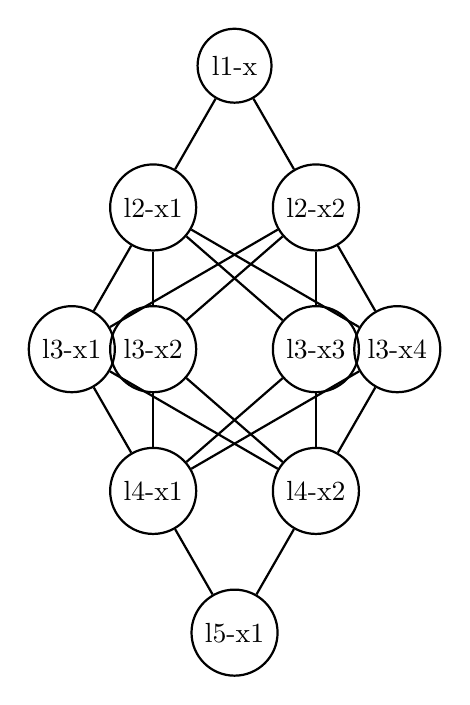
\begin{tikzpicture}\node[shape=circle,draw=black,align=center,line width=0.8pt] (0) at (6.233333333333333,14.866666666666667) {l1-x};
\node[shape=circle,draw=black,align=center,line width=0.8pt] (1) at (5.2,13.066666666666666) {l2-x1};
\node[shape=circle,draw=black,align=center,line width=0.8pt] (2) at (7.266666666666667,13.066666666666666) {l2-x2};
\node[shape=circle,draw=black,align=center,line width=0.8pt] (3) at (4.166666666666667,11.266666666666667) {l3-x1};
\node[shape=circle,draw=black,align=center,line width=0.8pt] (4) at (5.2,11.266666666666667) {l3-x2};
\node[shape=circle,draw=black,align=center,line width=0.8pt] (5) at (7.266666666666667,11.266666666666667) {l3-x3};
\node[shape=circle,draw=black,align=center,line width=0.8pt] (6) at (8.3,11.266666666666667) {l3-x4};
\node[shape=circle,draw=black,align=center,line width=0.8pt] (7) at (5.2,9.466666666666667) {l4-x1};
\node[shape=circle,draw=black,align=center,line width=0.8pt] (8) at (7.266666666666667,9.466666666666667) {l4-x2};
\node[shape=circle,draw=black,align=center,line width=0.8pt] (9) at (6.233333333333333,7.666666666666667) {l5-x1};

\path [-,draw=black,line width=0.8pt] (0) edge node {} (1);
\path [-,draw=black,line width=0.8pt] (1) edge node {} (3);
\path [-,draw=black,line width=0.8pt] (3) edge node {} (7);
\path [-,draw=black,line width=0.8pt] (7) edge node {} (9);
\path [-,draw=black,line width=0.8pt] (0) edge node {} (2);
\path [-,draw=black,line width=0.8pt] (2) edge node {} (6);
\path [-,draw=black,line width=0.8pt] (6) edge node {} (8);
\path [-,draw=black,line width=0.8pt] (8) edge node {} (9);
\path [-,draw=black,line width=0.8pt] (2) edge node {} (5);
\path [-,draw=black,line width=0.8pt] (5) edge node {} (8);
\path [-,draw=black,line width=0.8pt] (5) edge node {} (7);
\path [-,draw=black,line width=0.8pt] (6) edge node {} (7);
\path [-,draw=black,line width=0.8pt] (4) edge node {} (8);
\path [-,draw=black,line width=0.8pt] (3) edge node {} (8);
\path [-,draw=black,line width=0.8pt] (4) edge node {} (7);
\path [-,draw=black,line width=0.8pt] (2) edge node {} (4);
\path [-,draw=black,line width=0.8pt] (2) edge node {} (3);
\path [-,draw=black,line width=0.8pt] (1) edge node {} (4);
\path [-,draw=black,line width=0.8pt] (1) edge node {} (5);
\path [-,draw=black,line width=0.8pt] (1) edge node {} (6);
\end{tikzpicture}
\end{document}